\documentclass[11pt,a4paper]{report}
\usepackage[spanish,es-nodecimaldot]{babel}	% Utilizar español
\usepackage[utf8]{inputenc}					% Caracteres UTF-8
\usepackage{graphicx}						% Imagenes
\usepackage[hidelinks]{hyperref}			% Poner enlaces sin marcarlos en rojo
\usepackage{fancyhdr}						% Modificar encabezados y pies de pagina
\usepackage{float}							% Insertar figuras
\usepackage[textwidth=390pt]{geometry}		% Anchura de la pagina
\usepackage[nottoc]{tocbibind}				% Referencias (no incluir num pagina indice en Indice)
\usepackage{enumitem}						% Permitir enumerate con distintos simbolos
\usepackage[T1]{fontenc}					% Usar textsc en sections
\usepackage{amsmath}						% Símbolos matemáticos

% Comando para poner el nombre de la asignatura
\newcommand{\asignatura}{Simulación de sistemas}
\newcommand{\autor}{Adrián Acosa Sánchez}
\newcommand{\titulo}{PRÁCTICA 4}
\newcommand{\subtitulo}{Modelos de simulación dinámicos y continuos}
\newcommand{\rama}{Computación y Sistemas Inteligentes}

% Configuracion de encabezados y pies de pagina
\pagestyle{fancy}
\lhead{\autor{}}
\rhead{\asignatura{}}
\lfoot{Grado en Ingeniería Informática}
\cfoot{}
\rfoot{\thepage}
\renewcommand{\headrulewidth}{0.4pt}		% Linea cabeza de pagina
\renewcommand{\footrulewidth}{0.4pt}		% Linea pie de pagina

\usepackage{graphicx}
\begin{document}
\pagenumbering{gobble}

% Pagina de titulo
\begin{titlepage}

\begin{minipage}{\textwidth}

\centering

%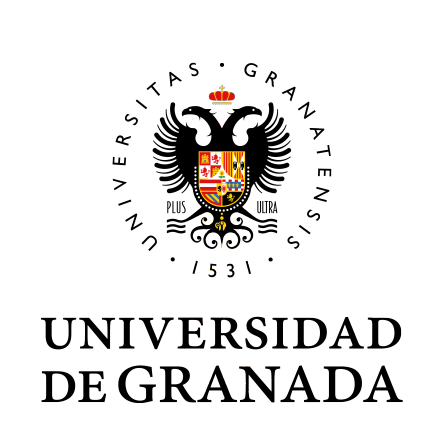
\includegraphics[scale=0.5]{img/ugr.png}\\

\includegraphics[scale=0.3]{img/logo_ugr.jpg}\\[1cm]

\textsc{\Large \asignatura{}\\[0.2cm]}
\textsc{GRADO EN INGENIERÍA INFORMÁTICA}\\[1cm]

\noindent\rule[-1ex]{\textwidth}{1pt}\\[1.5ex]
\textsc{{\Huge \titulo\\[0.5ex]}}
\textsc{{\Large \subtitulo\\}}
\noindent\rule[-1ex]{\textwidth}{2pt}\\[3.5ex]

\end{minipage}

%\vspace{0.5cm}
\vspace{0.7cm}

\begin{minipage}{\textwidth}

\centering

\textbf{Autor}\\ {\autor{}}\\[2.5ex]
\textbf{Rama}\\ {\rama}\\[2.5ex]
\vspace{0.3cm}


\includegraphics[scale=0.3]{img/etsiit.jpeg}

\vspace{0.7cm}
\textsc{Escuela Técnica Superior de Ingenierías Informática y de Telecomunicación}\\
\vspace{1cm}
\textsc{Curso 2022-2023}
\end{minipage}
\end{titlepage}

\pagenumbering{arabic}
\tableofcontents
\thispagestyle{empty}				% No usar estilo en la pagina de indice

\newpage

\setlength{\parskip}{1em}

\chapter{Propagación de una enfermedad infecciosa}

\newpage

\section{Simulaciones iniciales}

Para ponernos en situación, en esta práctica se nos plantea la simulación de la propagación de una enfermedad infecciosa (como podría ser el COVID-19) con el denominado modelo \textit{SIR}.

Vamos a tener en cuenta una población de \textit{N} individuos que podemos dividir en 3 grupos:

\begin{itemize}
	\item{Infectados o enfermos, $I(t)$, que tienen la enfermedad y pueden contagiarla.}
	\item{Susceptibles o propensos $S(t)$, que no tienen la enfermedad pero pueden contraerla.}
	\item{Retirados, $R(t)$, individuos que se han recuperado de la enfermedad (y ya no la contagian) y se han vuelto inmunes, o que han muerto.} 
\end{itemize}

En el guión se dan una serie de suposiciones que no voy a comentar aquí. La primera simulación que voy a ejecutar será con los parámetros de derivación $a=0.001$, $b=1/8$ (se recupera un infectado cada 8 días) y $c=1/180$.

Con estos datos, en las tareas que se proponen en el guión se pide observar qué ocurre si el número de individuos susceptibles es mayor o menor que $b/a$. En el caso de este ejemplo, el valor de $b/a$ es igual a 125, por lo tanto vamos a probar con un número de individuos susceptibles igual a 999 como se dice en la exposición del problema y tras esto vamos a ver qué pasa si usamos un número de individuos susceptibles igual a 100 para comparar los dos casos.

En primer lugar, todas las simulaciones las haré usando el método de Runge-Kutta con un $h=0.1$, y en el último apartado compararé el uso de el método de Euler y el de Runge-Kutta con distintos valores de $h$.

Para todas las simulaciones voy a coger 365 datos simulando un año de lapso de tiempo para ver mejor la evolución. En algunos casos dependerá de cómo evolucione cogeré más o menos datos en función de lo necesario.

\newpage
\subsection{Simulación con $S_0$ mayor que $b/a$}
\subsubsection{Con inmunidad permanente}

Veamos qué resultados hemos obtenemos con un $S_0$ igual a 999 con inmunidad permanente:

\begin{figure}[H]
\centering
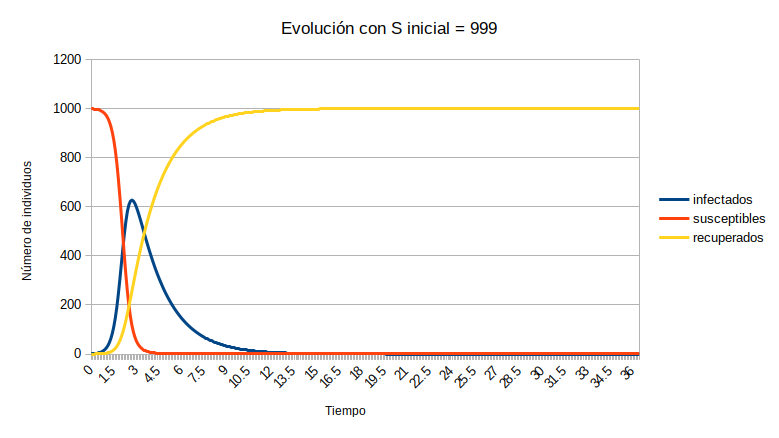
\includegraphics[width=\textwidth]{img/inmunidad/simulacion_ba_mayor.png}
\caption{Comparación de Infectados, Susceptibles y Recuperados en función del tiempo con $S_0$ mayor que $b/a$}
\label{}
\end{figure}

Podemos observar cómo los pacientes susceptibles de contagiarse decrecen su población muy rápidamente siendo contagiados todos ellos, lo que se ve reflejado en un pico ascendente en la gráfica de los infectados. A la vez que ocurre esto, también podemos ver como crece lentamente la gráfica de recuperados justo a la vez que los infectados decrecen muy rápidamente. Esta grafica tiene sentido ya que no se contempla la posiblidad de volver a contagiarse a la población que ya se ha recuprado de la infección, y por lo tanto casi en toda la gráfica podemos ver como toda la población ha pasado de susceptible a infectado, y de infectado a recuperado.

\newpage
\subsubsection{Sin inmunidad permanente}

Ahora vamos a ver qué cambia si añadimos el parámetro de la inmunidad no permanente con los mismos datos iniciales (he aumentado el número de días a 2 años):

\begin{figure}[htp]
\centering
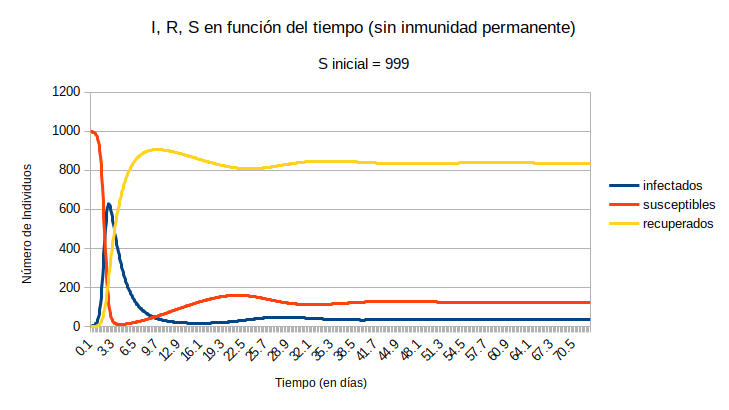
\includegraphics[width=\textwidth]{img/sin_inmunidad/simulacion_ba_mayor.png}
\caption{Infectados, Susceptibles y Recuperados en función del tiempo sin inmunidad permanente con $S_0$ es mayor que $b/a$}
\label{}
\end{figure}

La diferencia que existe en este caso entre la simulación con inmunidad permanente y sin inmunidad permanente es que el número de individuos de los tres grupos llega a estabilizarse a unos valores tras el pico, pero nunca llegan a quedarse todos los individuos en un grupo como pasa con la inmunidad permanente.

Vamos ahora a ver qué pasa con una población de susceptibles inicial menor que $b/a$.

\newpage
\subsection{Simulación con $S_0$ menor que $b/a$}
\subsubsection{Con inmunidad permanente}

Ahora vamos a ver que pasa cuando la población inicial de susceptibles es menor que $b/a$:

\begin{figure}[H]
\centering
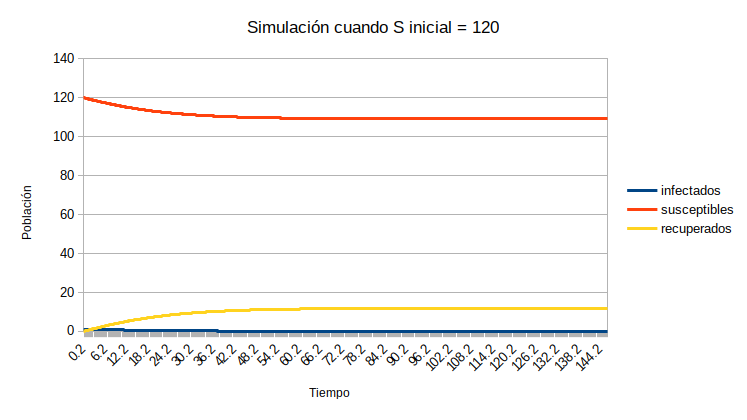
\includegraphics[width=\textwidth]{img/inmunidad/simulacion_ba_menor.png}
\caption{Comparación de Infectados, Susceptibles y Recuperados en función del tiempo con $S_0$ menor que $b/a$}
\label{}
\end{figure}

Esta vez para que se vea mejor la evolución de la población he usado un número de 4 veces más debido a que no se veía demasiado bien con 365 simulaciones. Se puede apreciar como el sistema tiende a equilibrarse y no hay un cambio tan brusco de Susceptibles a Recuperados pasando por Infectados. En este caso, el número de infectados se mantiene estable ya que como podemos ver que las curvas de Susceptibles y Recuperados son espejo una de la otra: cuando una tiene una curva descendente, la otra tiene una curva ascendente. Se puede sacar como conclusión que se debe a que no hay tanta población susceptible a la infección y por lo tanto el ratio de exposición es mucho menor que en el caso en el que tenemos 999 individuos susceptibles, que lo que ocurre es que al haber más personas expuestas se contagian más a la vez y estas a su vez a otras muchas más, descontrolando el contagio y provocando la curva vista en el apartado anterior.

\newpage
\subsubsection{Sin inmunidad permanente}
Ahora vamos a ver el mismo caso que en la página anterior pero teniendo inmunidad temporal:

\begin{figure}[H]
\centering
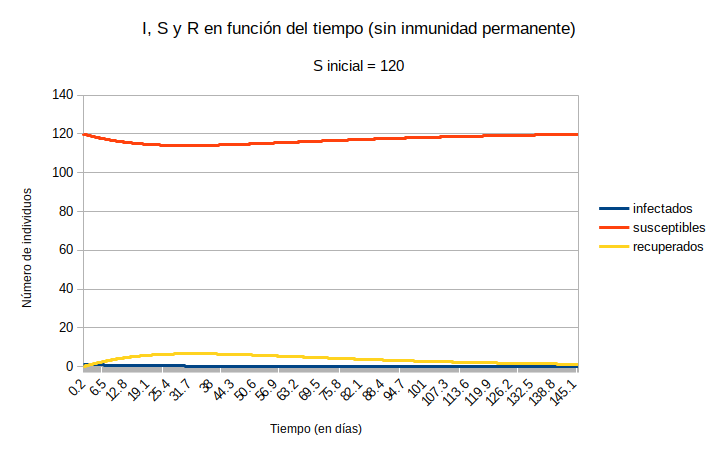
\includegraphics[width=\textwidth]{img/sin_inmunidad/simulacion_ba_menor.png}
\caption{Infectados, Susceptibles y Recuperados en función del tiempo sin inmunidad permanente con $S_0$ es menor que $b/a$}
\label{}
\end{figure}

Como se puede apreciar, en este caso la población de recuperados pasa a ser susceptibles casi completamente y los infectados llegan a ser 0. Es decir, pasa exactamente igual que en el caso anterior pero en este caso al perder la inmunidad en un cierto tiempo, todos los recuperados que había pasan a ser susceptibles en su totalidad.

\newpage
\section{Simulaciones alterando los parámetros de contacto, duración de la enfermedad e inmunidad.}

Para este apratado voy a usar sólamente la simulación donde se tiene inmunidad no permanente, ya que es donde mejor se van a ver las alteraciones porque si me limito a usar el modelo donde la inmunidad es permanente no se verá correctamente qué pasa si modifico el parámetro $c$. También voy a usar $N=1000$ para hacer las pruebas comenzando con un individuo infectado y el resto serán susceptibles.

\subsubsection{$a$ 10 veces mayor}

Por tanto vamos a ver qué pasa si modifico el parámetro $a$ y pongo un rango de exposición 10 veces más alto:

\begin{figure}[H]
\begin{tabular}{ll}
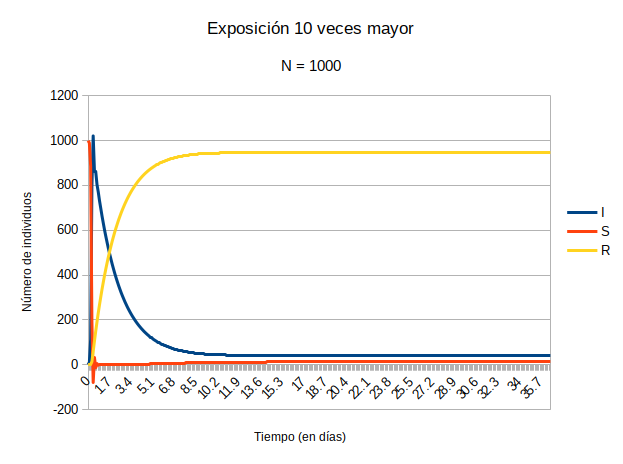
\includegraphics[scale=0.25]{img/sin_inmunidad/exposicion_x10.png}
&
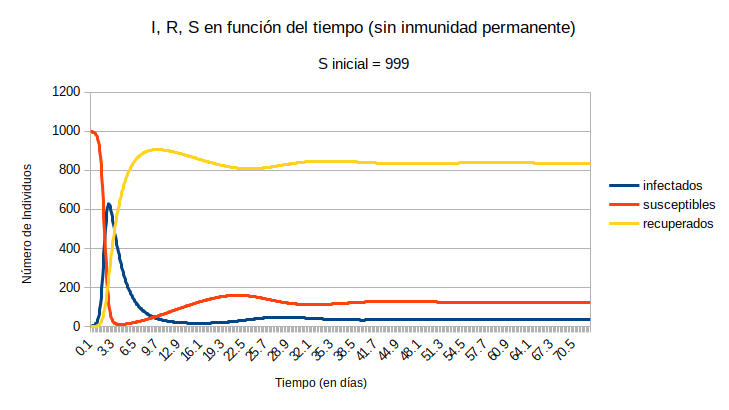
\includegraphics[scale=0.25]{img/sin_inmunidad/simulacion_ba_mayor.png}
\end{tabular}
\caption{Comparaciones entre las distintas situaciones posibles}
\end{figure}

Los dos cambios que se aprecian son que el contagio sucede muchísimo más deprisa en este caso y que los contagios y la recuperación suceden muy pareadas, es decir, se quedan constantes el número de susceptibles, infectados y recuperados como si se tratase del caso de la inmunidad permanente.

\subsubsection{$a$ 5 veces menor}

\begin{figure}[H]
\begin{tabular}{ll}
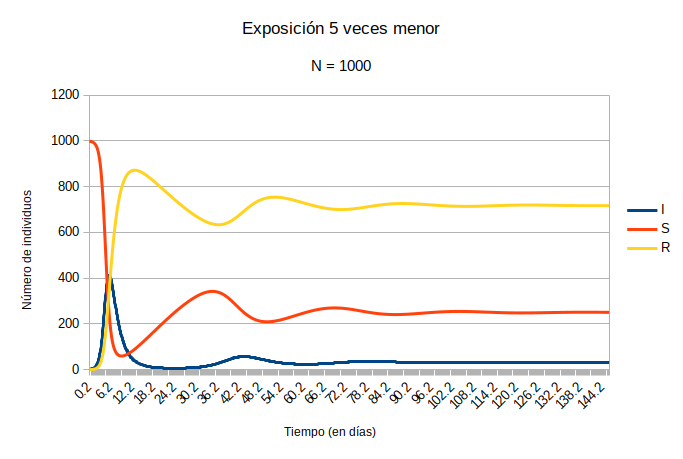
\includegraphics[scale=0.25]{img/sin_inmunidad/exposicion_x0_5.png}
&
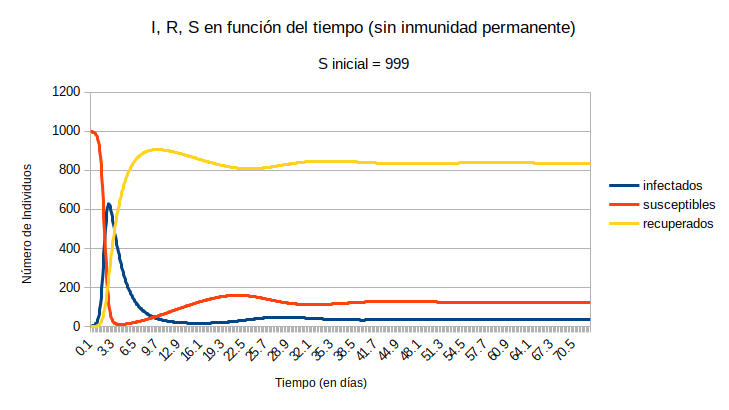
\includegraphics[scale=0.25]{img/sin_inmunidad/simulacion_ba_mayor.png}
\end{tabular}
\caption{Comparaciones entre las distintas situaciones posibles}
\end{figure}

Si disminuimos 5 veces el contagio, vemos como el pico de infectados es mucho menor y como va variando más el número de recuperados y susceptibles a lo largo del tiempo, es decir, tarda más en equilibrarse.

\subsubsection{Recuperación más lenta (16 días)}

Si aumentamos el número de días que tarda un individuo en recuperarse, obtenemos los siguientes datos:

\begin{figure}[H]
\begin{tabular}{ll}
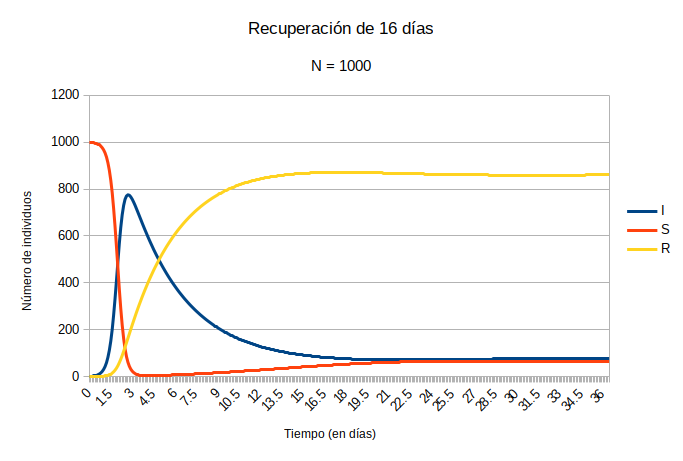
\includegraphics[scale=0.25]{img/sin_inmunidad/recuperacion_16dias.png}
&
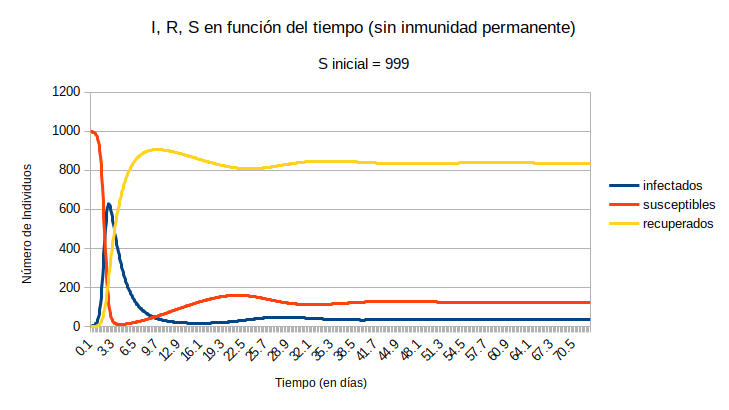
\includegraphics[scale=0.25]{img/sin_inmunidad/simulacion_ba_mayor.png}
\end{tabular}
\caption{Comparaciones entre las distintas situaciones posibles}
\end{figure}

Como se puede apreciar en la línea amarilla, la curva es mucho menos pronunciada en el caso de que la recuperación sea más lenta, además de que la curva de infectados es un poco más amplia debido al mismo motivo.

\subsubsection{Inmunidad mucho menos tiempo, recuperación más lenta e infección mayor}

Vamos a ver que pasa si combinar un menor tiempo de inmunidad (sólo 10 días de inmunidad) con un mayor ratio de infección (10 veces mayor) y con una recuperación más lenta (10 días):

\begin{figure}[H]
\centering
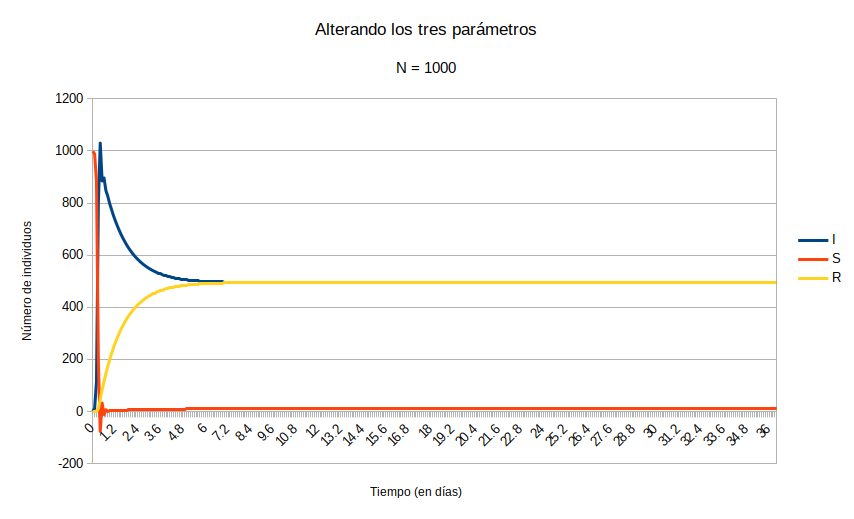
\includegraphics[width=\textwidth]{img/sin_inmunidad/alterado_all.png}
\caption{Alterando todos los estados}
\label{}
\end{figure}

Aquí se puede apreciar que alterando todos los parámetros tal y como se comenta en el primer párrafo, no da tiempo a que los individuos pasen mucho tiempo en susceptibles al perder la inmuidad muy rápido. Se ve reflejado en la gráfica con la superposición de los infectados con los recuperados, ya que en el momento en que los recuperados van a pasar a ser susceptibles, se infectan rápidamente.

\newpage
\section{Alterando los valores de población iniciales}

Voy a seguir con el modelo donde los recuperados pierden la inmunidad cada cierto tiempo y voy a usar los parámetros del principio de las simulaciones ($N = 1000$).

Voy a realizar las siguientes tres pruebas:

\begin{itemize}
	\item 100 infectados, 800 susceptibles y 100 recuperados
	\item 500 infectados, 500 susceptibles y 0 recuperados
	\item 400 infectados, 400 susceptibles y 200 recuperados
\end{itemize}

Veamos que pasa en los siguientes apartados.

\newpage
\subsubsection{Primer caso}

La simulación del primer punto da como resultado la siguiente gráfica:

\begin{figure}[H]
\centering
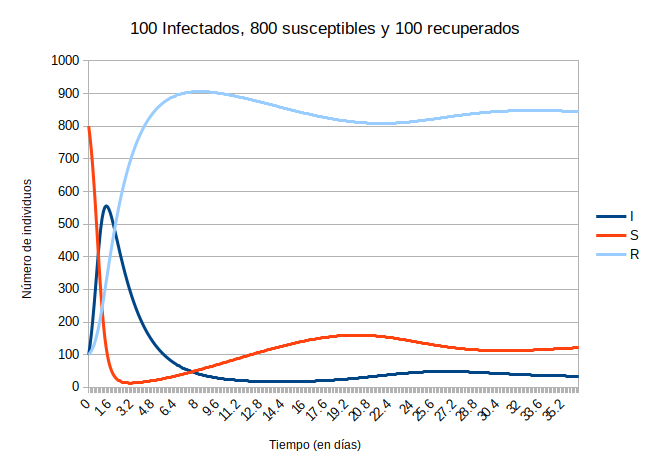
\includegraphics[width=\textwidth]{img/sin_inmunidad/100i_800s_100r.png}
\caption{Simulación del primer caso}
\label{}
\end{figure}

En este caso no hay demasiadas diferencias con los otros casos, salvo en los valores iniciales y en lo que van variando las gráficas. Vamos a ver qué pasa con el siguiente caso.

\newpage
\subsubsection{Segundo caso}

\begin{figure}[H]
\centering
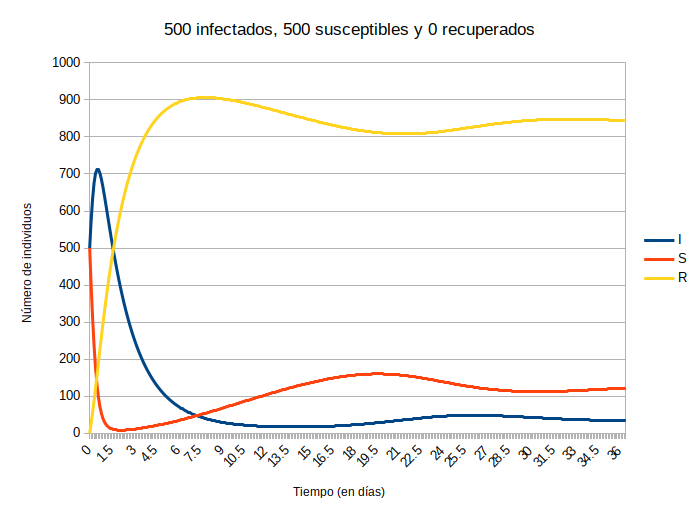
\includegraphics[width=\textwidth]{img/sin_inmunidad/500i_500s_0r.png}
\caption{Resultados del segundo caso}
\label{}
\end{figure}

Tampoco vemos una diferencia muy grande salvo que la gráfica se ve desplazada hacia la izquierda.

\newpage
\subsubsection{Tercer caso}

\begin{figure}[H]
\centering
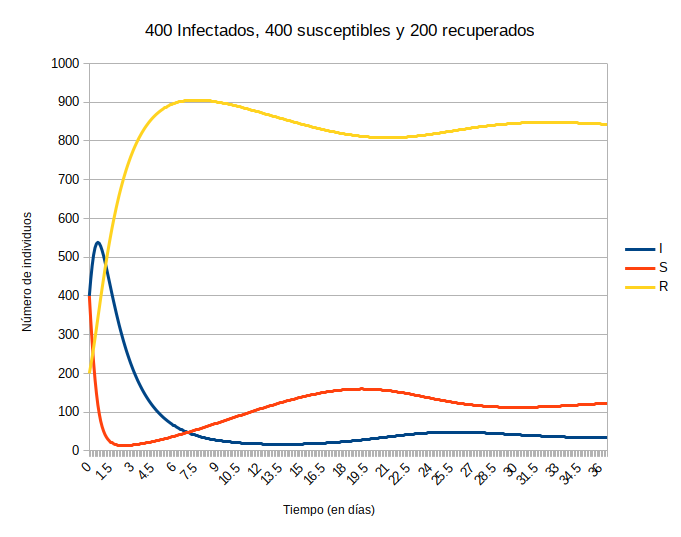
\includegraphics[width=\textwidth]{img/sin_inmunidad/400i_400s_200r.png}
\caption{Resultados del tercer caso}
\label{}
\end{figure}

Pasa lo mismo que en los dos casos anteriores. Es como si la gráfica estuviese desplazada. 

\subsubsection{Conclusión}

Como conclusión podemos sacar que el número de individuos iniciales perteneciente a cada uno de los grupos no es tan relevante como el ajustar los parámetros $a$, $b$ y $c$, que obviamente marcan una diferencia significativa en los resultados ya que son los que controlan el tiempo de recuperación de un individuo, el ratio de exposición ante la infección y el tiempo que tarda en perder la inmunidad. Estos parámetros son mucho más importantes a la hora de ver los resultados que el número de individuos que pertenecen a cada grupo.


\newpage
\section{Comparación entre métodos de Runge-Kutta y Euler}

Como último estudio a realizar, en el guión se pide que se comparen los métodos de Runge-Kutta y de Euler. Para ello vamos a diferenciar entre el caso de inmunidad permanente y el de no permanente. En primer lugar vamos con el de inmunidad permantente. Sobre todo probaré el método de Euler ya que sólo lo voy a usar en este apartado.

\subsubsection{Con inmunidad permanente}

Vamos a comparar el caso de la simulación inicial con los dos métodos de cálculo: 

\begin{figure}[H]
\begin{tabular}{ll}
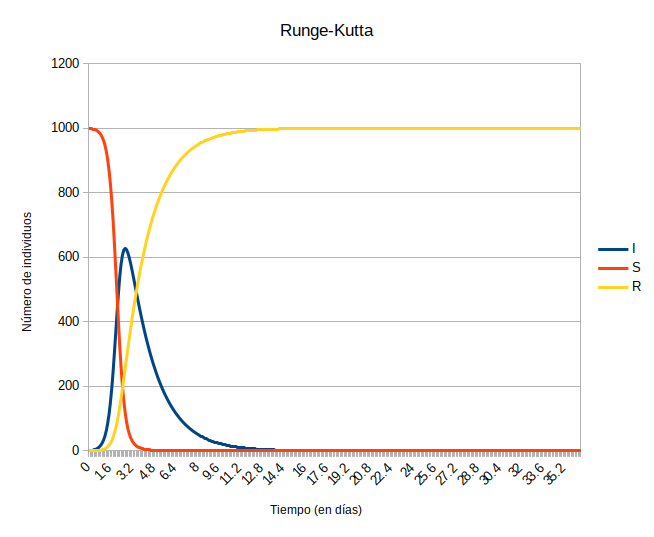
\includegraphics[scale=0.25]{img/inmunidad/runge-kutta.png}
&
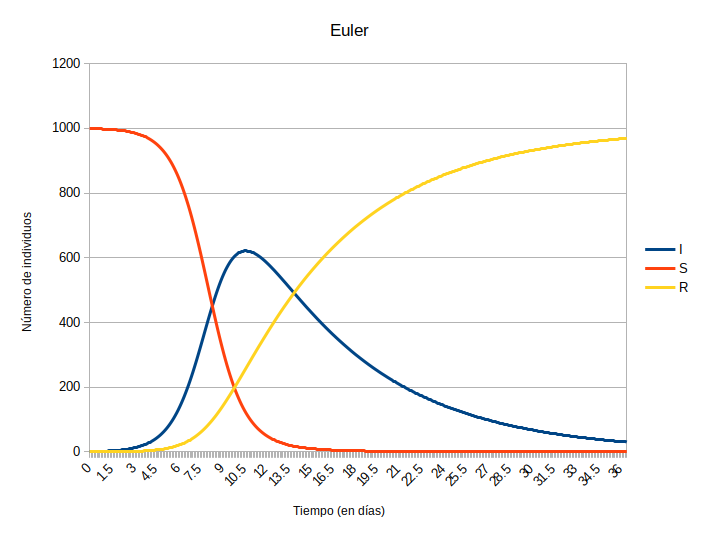
\includegraphics[scale=0.25]{img/inmunidad/euler.png}
\end{tabular}
\caption{Comparacion entre los métodos de Euler y Runge-Kutta}
\end{figure}

La diferencia más notoria es que el método de Euler da unos resultados mucho más espaciados, es decir, da los mismos valores pero si nos fijamos en el pico de infectados se encuentra desplazado hacia la derecha.

Vamos a comparar qué pasa si cambiamos $h = 0,05$:

\begin{figure}[H]
\begin{tabular}{ll}
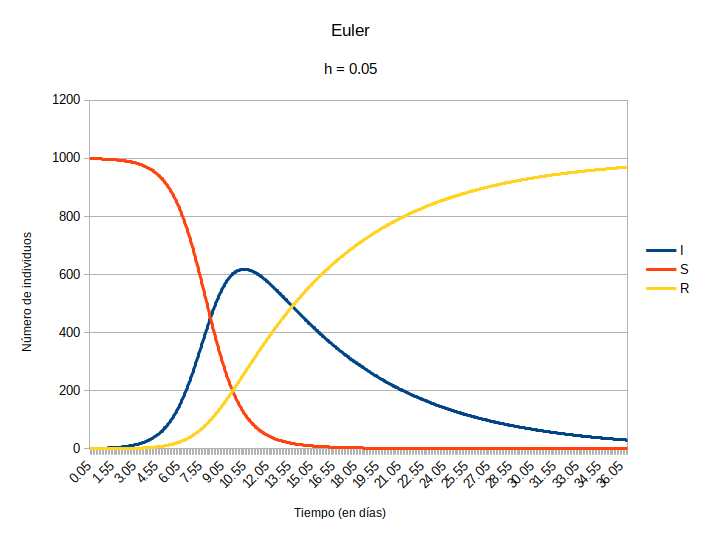
\includegraphics[scale=0.25]{img/inmunidad/euler-0-5.png}
&
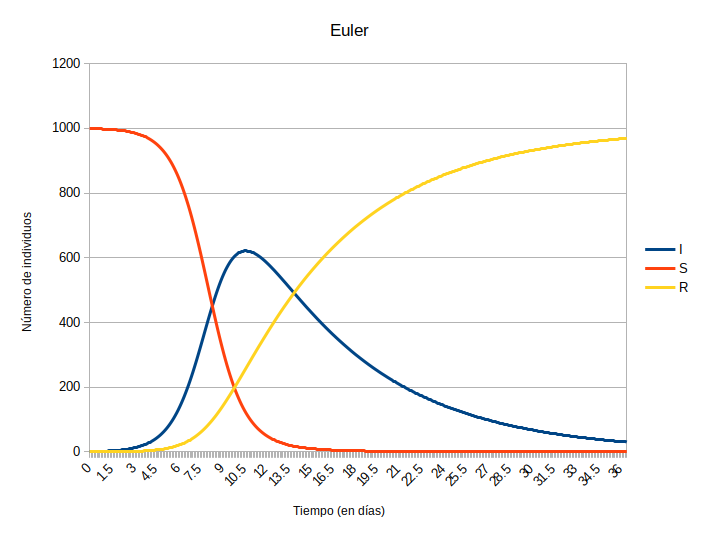
\includegraphics[scale=0.25]{img/inmunidad/euler.png}
\end{tabular}
\caption{Comparacion entre los métodos de Euler con $h = 0,05$ y $h = 0,1$}
\end{figure}

La diferencia es inapreciable, la diferencia está en la precisión de los cálculos.

\begin{figure}[H]
\begin{tabular}{ll}
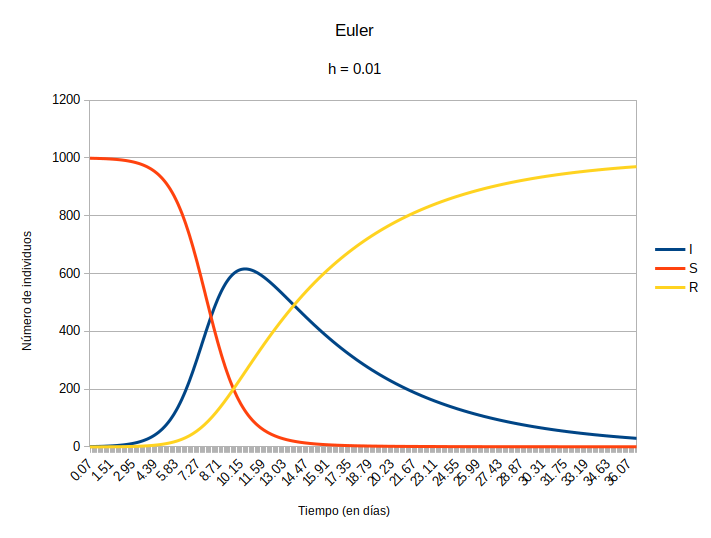
\includegraphics[scale=0.25]{img/inmunidad/euler-0-01.png}
&
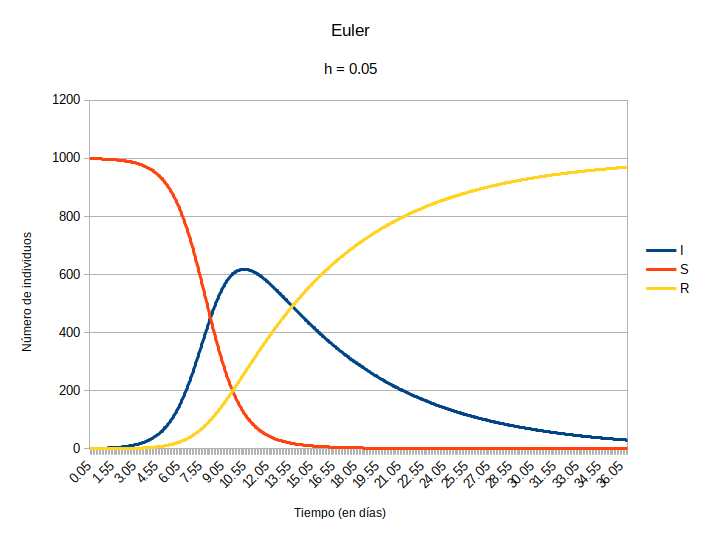
\includegraphics[scale=0.25]{img/inmunidad/euler-0-5.png}
\end{tabular}
\caption{Comparacion entre los métodos de Euler con $h = 0,01$ y $h = 0,05$}
\end{figure}

\newpage
\subsubsection{Sin inmunidad permanente}

Vamos a comparar Runge-Kutta con Euler en el caso de la inmunidad no permanente:

\begin{figure}[H]
\begin{tabular}{ll}
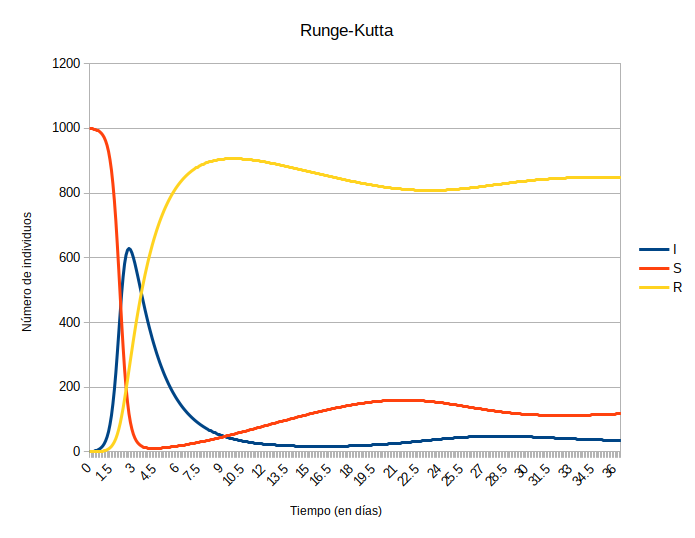
\includegraphics[scale=0.25]{img/sin_inmunidad/runge-kutta.png}
&
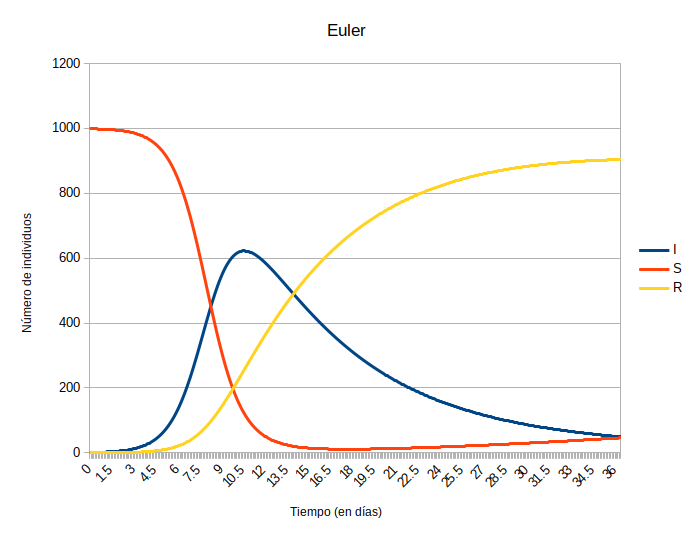
\includegraphics[scale=0.25]{img/sin_inmunidad/euler.png}
\end{tabular}
\caption{Comparacion entre los métodos de Euler y Runge-Kutta}
\end{figure}

Pasa exactamente lo mismo que en el caso de inmunidad permanente.

Vamos a comparar el método de euler para los distintos valores de $h$ tal y como lo he hecho para la inmunidad permanente:

\begin{figure}[H]
\begin{tabular}{ll}
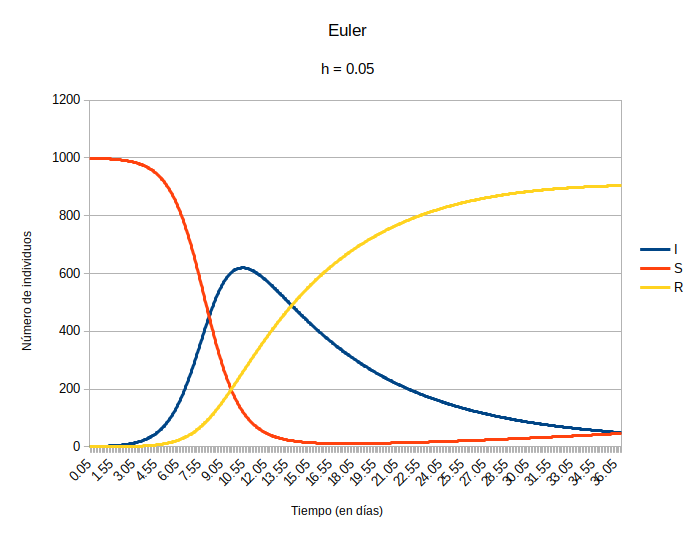
\includegraphics[scale=0.25]{img/sin_inmunidad/euler-0-05.png}
&
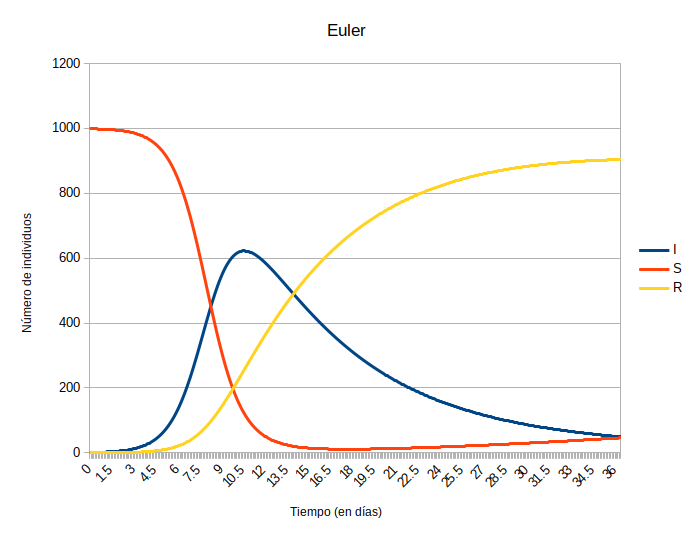
\includegraphics[scale=0.25]{img/sin_inmunidad/euler.png}
\end{tabular}
\caption{Comparacion entre los métodos de Euler con $h = 0,05$ y $h = 0,1$}
\end{figure}

\begin{figure}[H]
\begin{tabular}{ll}
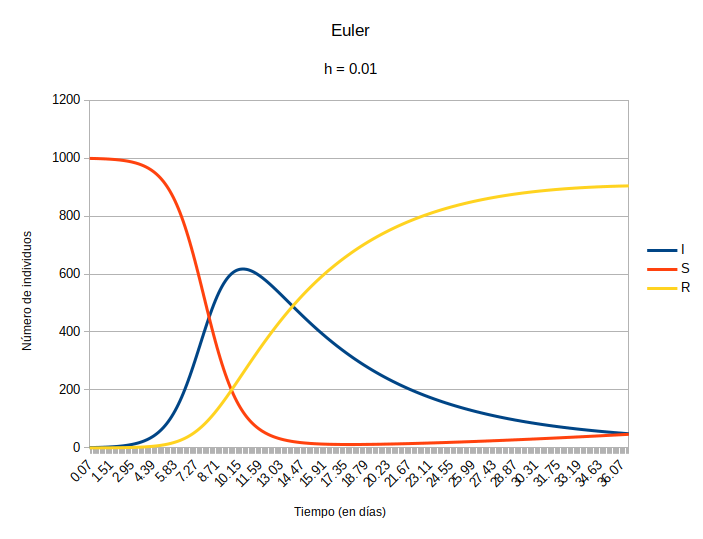
\includegraphics[scale=0.25]{img/sin_inmunidad/euler-0-01.png}
&
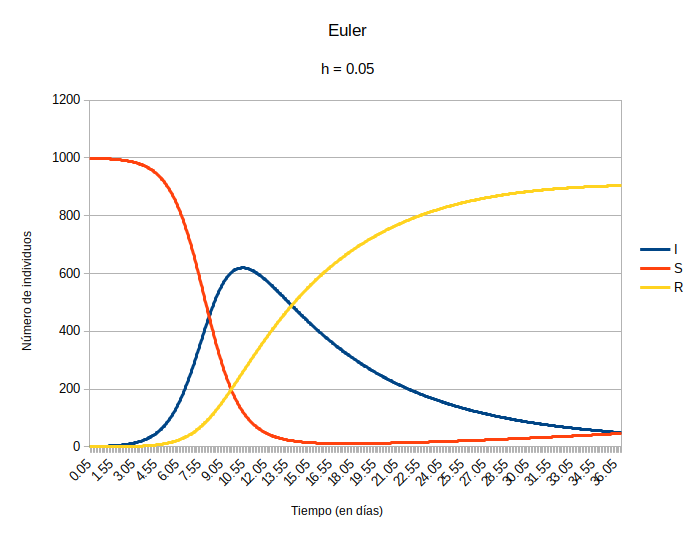
\includegraphics[scale=0.25]{img/sin_inmunidad/euler-0-05.png}
\end{tabular}
\caption{Comparacion entre los métodos de Euler con $h = 0,01$ y $h = 0,05$}
\end{figure}

\subsubsection{Conclusión}

Si queremos unos valores de cálculo más precisos, lo que tendremos que hacer es bajar el parámetro $h$ tanto como precisión queramos tener. El método que queramos elegir para realizar éstos cálculos dependerá de nuestros gustos también.

\end{document}

